\documentclass{amsart}
\usepackage{amsfonts, amsthm, amssymb, amsmath}
\usepackage{mathtools}
\usepackage{graphicx,caption,subcaption}
\usepackage{comment}
\usepackage{xcolor}
\usepackage{tikz}
%\usetikzlibrary{decorations.markings,arrows.meta,calc,fit,quotes,cd,math,external}
\usetikzlibrary{
  matrix,
  arrows,
  arrows.meta,
  calc,
  fit,
  quotes,
  cd,
  math,
  external,
  shapes,
  decorations.markings,
  decorations.pathreplacing,
  patterns,
  decorations.pathmorphing
}

\usepackage{url}
\usepackage[inline]{enumitem}
	\setlist{itemsep=0em, topsep=0em, parsep=0em}
	\setlist[enumerate]{label=(\alph*)}
\usepackage[all,2cell]{xy}\UseAllTwocells\SilentMatrices
\usepackage[breaklinks=true]{hyperref}%John's choices, can change; previous choice \definecolor{hyperrefcolor}{rgb}{0,0,0.7}
\definecolor{darkgreen}{rgb}{0,0.45,0}
\definecolor{myurlcolor}{rgb}{0.6,0,0}
\definecolor{mycitecolor}{rgb}{0,0,0.8}
\definecolor{myrefcolor}{rgb}{0,0,0.8}
\hypersetup{colorlinks, linkcolor=myrefcolor, citecolor=darkgreen, urlcolor=myurlcolor,
final,linktoc=page}
\usepackage[capitalize]{cleveref}
\crefname{equation}{}{}
\crefname{item}{}{}
\crefname{prop}{Proposition}{Propositions}

%
% environments and counters
%

\newtheorem{thm}{Theorem}[section]
\newtheorem{cnj}[thm]{Conjecture}
\newtheorem{lem}[thm]{Lemma}
\newtheorem{prop}[thm]{Proposition}
\newtheorem{cor}[thm]{Corollary}

\theoremstyle{remark}
	\newtheorem{remark}[thm]{Remark}
	\newtheorem{notation}[thm]{Notation}

\theoremstyle{definition}
	\newtheorem{ex}[thm]{Example} 
	\newtheorem{defn}[thm]{Definition}

% math text formatting
\newcommand{\cat}[1]{\mathsf{#1}}

% common category names

\newcommand{\Set}{\cat{Set}}
\newcommand{\Grph}{\cat{Grph}}
\newcommand{\Cat}{\cat{Cat}}
\newcommand{\twoCat}{\cat{2Cat}}
\newcommand{\Adj}{\cat{Adj}}
\newcommand{\one}{\mathbf{1}}
\newcommand{\two}{\mathbf{2}}
\newcommand{\Fib}{\cat{Fib}}
\newcommand{\OpFib}{\cat{OpFib}}
\newcommand{\Corefl}{\cat{Corefl}}
\newcommand{\Rali}{\cat{Rali}}

\newcommand{\C}{\cat{A}}
\newcommand{\D}{\cat{X}}
\newcommand{\A}{\cat{A}}
\newcommand{\X}{\cat{X}}
\newcommand{\U}{U}
\newcommand{\Q}{Q}
\renewcommand{\L}{L}
\newcommand{\R}{R}
\renewcommand{\P}{P}
\newcommand{\B}{\cat{B}}
\newcommand{\Y}{\cat{Y}}

\newcommand{\Cocart}{\mathrm{Cocart}}
\newcommand{\Cart}{\mathrm{Cart}}

\newcommand{\op}[1]{\operatorname{#1}}
\renewcommand{\t}[1]{\text{#1}}

\newcommand{\from}{\colon}
\newcommand{\xto}[1]{\xrightarrow{#1}}
\newcommand{\To}{\Rightarrow}
\newcommand{\Tto}{\Rrightarrow}
\newcommand{\bydef}{\coloneqq}
\newcommand{\define}{\textbf}%consider change to bold? or something else?

%
% math operators
%

\DeclareMathOperator{\Hom}{Hom}
\DeclareMathOperator{\id}{id}
\DeclareMathOperator{\ob}{Ob}
\DeclareMathOperator{\arr}{arr}
\DeclareMathOperator{\im}{im}
\DeclareMathOperator{\Aut}{Aut}
\DeclareMathOperator{\Bij}{Bij}
\DeclareMathOperator{\Sub}{Sub}
\DeclareMathOperator{\colim}{colim}
\newcommand{\iso}{\cong}

%
% tikz styles
%

% arrows for commuting diagram
\tikzset{
  cd/.style={
    ->,
    scale=6,
    >=angle 90,
    font=\scriptsize}
  }

% its us!

\definecolor{purple(x11)}{rgb}{0.5, 0.0, 0.5}
\newcommand{\chris}{\color{purple(x11)}}
\newcommand{\daniel}{\color{red}}


\newcommand{\nice}{\emph{nice}}

\begin{document}
\title{Fibrations and Adjunctions}

\author{Daniel Cicala and Christina Vasilakopoulou} 
\address{Departement of Mathematics, University of California, Riverside, 900 University Avenue, 92521, USA}
\email{cicala@math.ucr.edu,vasilak@ucr.edu}

\begin{abstract}
Fibrations and Adjunctions rock.
\end{abstract}

\maketitle

\tableofcontents

\section{Introduction}

\section{Preliminaries}

Mainly basics of fibrations and adjunctions, to fix terminology. Also Street stuff.

\section{Sth}
Gray's and our theorem as one big thing. Maybe start from Street, and restrict to Grothendieck.

Then, monoidal analogue.

Then, probably lift to (2-)categories of such things.

[Here probably ends more or less what is needed for network big picture. Surely we can think of other things we wanna say.]

%We are closing in on a pair of theorems.

%\begin{thm}
%	Fix an adjunction 
%	\[
%	\begin{tikzpicture}
%		\node (C) at (0,0) {$ C $}	;
%		\node (D) at (2,0) {$ D $}	;
%		\draw [->] (C.30) to node {$ L $} (D.150);
%		\draw [->] (D.210) to node [swap] {$ R $} (C.-30);
%	\end{tikzpicture}
%	\]
%	$ R $ is a Street opfibration if and only if the adjunction in \nice.	
%\end{thm}

\begin{thm}
	Let $ \D $ have pushouts. Given a coreflection $ L \dashv R \from \C \to \D $ where $ R $ preserves pushouts, $ R $ is a Street opfibration.
\end{thm}

\begin{proof}
	Fix an arrow $ f \from a \to b $ in $ \C $ and an object $ x $ such that $ Rx \bydef a $.  Define $ \hat{f} $ as the pushout of $ Lf $ along the counit $ \epsilon_x $
	\[
	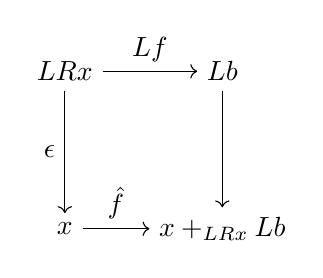
\begin{tikzpicture}
		\node (ul) at (0,2) {$ LRx $};
		\node (ll) at (0,0) {$ x $};
		\node (ur) at (2,2) {$ Lb $};
		\node (lr) at (2,0) {$ x +_{LRx} Lb$};
		\draw [->] (ul) to node [left] {$ \epsilon $} (ll);
		\draw [->] (ul) to node [above] {$ Lf $} (ur);
		\draw [->] (ll) to node [above] {$ \hat{f} $} (lr);
		\draw [->] (ur) to (lr);
	\end{tikzpicture}
	\] 
	Observe that $ R \hat{f} \from Rx \to R( x +_{LRx} Lb ) $. Also there is a string of isomorphisms  
	\[
		R( x +_{LRx} Lb ) \to Rx +_{RLRx} RLb \to Rx +_{Rx} b \to b
	\]
	whose composite we call $ h $. Then $ R \hat{f} = f . h^{-1} $ as desired.  \emph{(note: some details are needed here)}
	
	Now show that $ \hat{f} $ is cocartesian.  Consider a $ \D $-arrow $ g \from x \to y $ with a $ C $-arrow $ \theta \from R( x +_{LRx} Lb ) \to Ry  $ so that $ R \hat{f} . \theta = Rg $.  Can we uniquely lift $ \theta $? Set up the diagram
	\[
	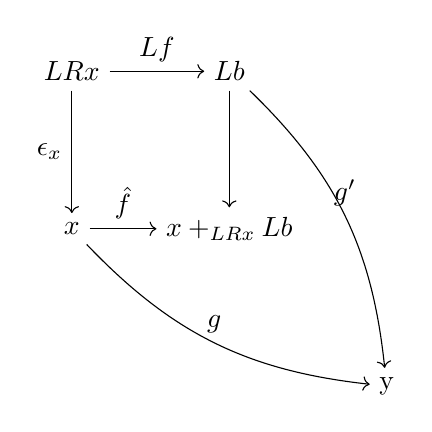
\begin{tikzpicture}
		\node (ul) at (0,2) {$ LRx $};
		\node (ll) at (0,0) {$ x $};
		\node (ur) at (2,2) {$ Lb $};
		\node (lr) at (2,0) {$ x +_{LRx} Lb$};
		\node (comp) at (4,-2) {y};
		\draw [->] (ul) to node [left] {$ \epsilon_x $} (ll);
		\draw [->] (ul) to node [above] {$ Lf $} (ur);
		\draw [->] (ll) to node [above] {$ \hat{f} $} (lr);
		\draw [->] (ur) to (lr);
		\draw [->] (ll) to [bend right=20] node [above] {$ g $} (comp);
		\draw [->] (ur) to [bend left=20] node [above] {$ g' $} (comp);
	\end{tikzpicture}
	\] 
	where $ g' \bydef Lh^{-1} . L\theta.\epsilon_y $.  To show the outer square commutes, it suffices to show that $ Lf . g' $ and $ \epsilon_x . g $ have the same image under the adjunction homset correspondence.  We have
	\[
		Lf . g' = Lf . Lh^{-1} . L\theta.\epsilon_y 
			\mapsto \eta_{Rx} . RLf . RLh^{-1} . RL\theta.R\epsilon_y 
			= f . h^{-1} . \theta  
			= R \hat{f} . \theta 
			= Rg
	\]
	and 
	\[
	\epsilon_x . g \mapsto \eta_{Rx} . Rg = Rg.	
	\]
\end{proof}

Perhaps it will be helpful to also tackle the special case of Grothendieck fibrations.

\begin{cnj}
If $\cat{C}$ and $\cat{D}$ have chosen pushouts (where a pushout of a morphism $f$ along the
identity `is' $f$) such that $R\colon\cat{D}\to\cat{C}$ strictly preserves them, then $R$ is an opfibration
when $R$ is a lari.
\end{cnj}

\begin{proof}
{\chris Wait for Lack's response to untangle the mess with chosen limits and colimits, and preserving them}
\end{proof}

For the converse, Gray already gives an answer for the Grothendieck case.

\begin{thm}
 {\chris write Gray and proof. Looks like choice issues are better understood here.}
\end{thm}

For the Street case, we can 'relax' the above, or go to a different direction as below. {(\chris write the relaxed Gray as well)}

\begin{thm}
	Given a Street opfibration $ R \from \cat{D} \to \cat{C} $, it is a right adjoint when it is \nice.
\end{thm}
 
Let's try to figure out what \nice could be. Here are some helpful theorems.

\begin{thm}[Freyd's general adjoint functor theorem]
\label{thm:GAFT}
	A functor $ F \from X \to Y $ is a right adjoint if  $ x $ is complete, locally small, and $ F $ satisfies the \emph{solution set condition}. The latter says, for any $ Y $-object $ y $, there exists a small set $ I $ indexing a collection of $ X $-objects $ {x_i}_I $ and $ Y $-arrows $ {f_i \from y \to F ( x_i ) } $ such that every $ F $-valued $ Y $-arrow $ y \to R x $ factors as $ Fg . f_k $ for $ k \in I $ and $ g \from x_k \to x $.
\end{thm}

\begin{thm}[Gabriel-Zisman]
\label{thm:GabZis}
	An adjunction $ L \dashv R \from \cat{C} \leftrightarrow \cat{D} $. TFAE:
	\begin{enumerate}
		\item $ L $ is full and faithful;
		\item the unit is an isomorphism;
		\item the induced comonad on $ \cat{D} $ is idempotent, $ L $ is conservative, and $ R $ is essentially surjective.
	\end{enumerate}
\end{thm}

Now, let's prove a strong theorem then try to weaken it

\begin{thm}
	Let $ \cat{D}$ be locally small and complete. Also let $ R \from \cat{D} \to \cat{C} $ be a continuous, surjective-on-objects Grothendiek opfibration.  Then $ R $ is a right adjoint.
\end{thm}

\begin{proof}
	We use \ref{thm:GAFT}.  Suffice to show the solution set condition holds.  Fix a $ C $-objects $ c $.  Then the indexing set is $ \ast $, the collection of $ D $-objects consists of a single object $ x_c $ over $ c $ (which exists by surjective-on-objects assumption), and the collection of $ \cat{C} $-arrows consists of the identity.  Any map $ f \from c \to Rd $ has a cocartesian lifting $ \hat{f} \from x_c \to x_{Rd} $ and $ f = R \hat{f} . 1_c $.
\end{proof}

\begin{thm}
	Let $ \cat{D}$ be locally small and complete. Also let $ R \from \cat{D} \to \cat{C} $ be a continuous, surjective-on-objects, conservative Street opfibration.  Then $ R $ is a right adjoint.
\end{thm}

\begin{proof}
	We use \ref{thm:GAFT}.  Suffice to show the solution set condition holds.  Fix a $ C $-objects $ c $.  Then the indexing set is $ \ast $, the collection of $ D $-objects consists of a single object $ x_c $ over $ c $ (which exists by surjective-on-objects assumption), and the collection of $ \cat{C} $-arrows consists of the identity.  For any map $ f \from c \to Rd $, there exists an essential cocartesian lifting $ \hat{f} \from x_c \to d' $ together with a $ \cat{C} $-isomorphism $ h \from Rd' \to Rd $ such that $ f = h . R \hat{f} $. But $ f = h . R \hat{f} = R \hat{h} . R \hat{f} . 1_c = R (\hat{h} . \hat{f}) . 1_c $ where $ h = R \hat{h} $ because $ R $ is conservative.
\end{proof}

\begin{thm}
	Let $ \cat{D}$ be locally small and complete. Also let $ R \from \cat{D} \to \cat{C} $ be a continuous, essentially surjective, conservative Street opfibration.  Then $ R $ is a right adjoint.
\end{thm}

\begin{proof}
	We use \ref{thm:GAFT}.  Suffice to show the solution set condition holds.  Fix a $ C $-object $ c $.  Then the indexing set is $ \ast $, the collection of $ D $-objects consists of a single object $ d' $ where $ \theta \from c \cong Rd' $ (which exists by essential surjectivity), and the collection of $ \cat{C} $-arrows is $ { \theta } $.  For any $ \cat{C} $-arrow $ f \from c \to Rd $, we have (by Street opfibrationness) $ f . \theta^{-1} \from Rd' \to c \to Rd $, a cocartesian essential lifting $ \hat{ f . \theta^{-1} } \from d' \to d'' $ in $ \cat{D} $, and an isomorphism $ h \from d \to d'' $ (by conservatism) such that $ f . \theta^{-1} = Rh . R \hat{ f . \theta^{-1} } $.  This implies, as required by GAFT, that $ f = R (h\hat{ f . \theta }) . \theta $.
\end{proof}

Thoughts about these assumptions. Here are the desired examples I can think of now: $ \cat{Set} $ together with $ \cat{Graph} $ or $ \cat{Top} $. The enriched over sets and completeness are both there. So is essential surjectivity. And reflection of isomorphisms.  The continuity is definitely needed, since it's necessary if $ R $ is a right adjoint. 

Go back to the right adjoint we had in the ``converse'' to the above theorem.  That is, we have a coreflection $ L \dashv R \from \cat{C} \leftrightarrow \cat{D} $ where $ L $ is left exact.  Of course this gives the continuity of $ R $. Essential surjectivity follows from Gabriel-Zisman. Is it a Street opfibration? $ L $ is conservative, but is $ R $?

\begin{ex}
	No, $ R $ is not in general conservative.  Consider the underlying node functor $ \Graph \to \Set $.  All $ \Graph $-endomorphisms on
	\[
	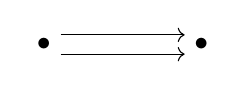
\begin{tikzpicture}
		\node (a) at (0,0) {$ \bullet $};
		\node (b) at (2,0) {$ \bullet $};
		\draw [->] (a.30) to (b.150);
		\draw [->] (a.-30) to (b.-150);
	\end{tikzpicture}
	\]
	are sent to the identity on $ 2 $.
\end{ex}

At this point, we have partial converses:

\fbox{
\begin{minipage}{0.4\textwidth}
		Let $ \D $ have pushouts. Given a coreflection $ L \dashv R \from \C \to \D $ where $ R $ preserves pushouts, $ R $ is a Street opfibration.
\end{minipage}
}
\hfill
\fbox{
\begin{minipage}{0.4\textwidth}
		Let $ \cat{D}$ be locally small and complete. Also let $ R \from \cat{D} \to \cat{C} $ be a continuous, essentially surjective, conservative Street opfibration.  Then $ R $ is a right adjoint.
\end{minipage}
}



































\end{document}

